\documentclass{report}

\usepackage{hyperref}

\usepackage{epstopdf}
\usepackage{amsmath}
\usepackage{amssymb}
\usepackage{subfig}
%\usepackage{multirow}
\usepackage[utf8]{inputenc}
\usepackage[T1]{fontenc}
\usepackage{standalone}
\usepackage{tikz}
\usepackage{tabularx}
\usepackage{float}
\usepackage[section]{placeins}
\usepackage{sverb}
\usepackage{import}
\usepackage{verbatim}
\usepackage{listings}
\usepackage{xcolor}

\graphicspath{{img/}}
\DeclareGraphicsExtensions{.pdf,.png,.jpg,.svg} %For pdflatex






\definecolor{codegreen}{rgb}{0,0.6,0}
\definecolor{codegray}{rgb}{0.5,0.5,0.5}
\definecolor{codepurple}{rgb}{0.58,0,0.82}
\definecolor{backcolour}{rgb}{0.95,0.95,0.92}

\lstdefinestyle{mystyle}{
    backgroundcolor=\color{backcolour},   
    commentstyle=\color{codegreen},
    keywordstyle=\color{magenta},
    numberstyle=\tiny\color{codegray},
    stringstyle=\color{codepurple},
    basicstyle=\ttfamily\footnotesize,
    breakatwhitespace=false,         
    breaklines=true,                 
    captionpos=b,                    
    keepspaces=true,                 
    numbers=left,                    
    numbersep=5pt,                  
    showspaces=false,                
    showstringspaces=false,
    showtabs=false,                  
    tabsize=2,
    float=H,
    extendedchars=\true, 
}


\lstset{style=mystyle}


\begin{document}

\begin{titlepage}
    \begin{center}
        
\includegraphics[width=.50\linewidth]{other/polsl.png}\\
        \Huge
        \textbf{Przetwarzanie Obrazów Cyfrowych}
        \\ \vspace{1.5cm}
        \Large
        \textbf{Raport z ćwiczenia nr. 1: } \\
        % \textbf{WSTĘPNE PRZETWARZANIE OBRAZÓW — FILTRY LINIOWE}
        \textbf{Filtry nieliniowe}        
    \end{center}
    \vspace{3.0cm}
    \Large
    Raport opracował: \\
    Dawid Kania \\
    Grupa 6 Semestr 7 \\ \\
    Data wykonania ćwiczenia: 17.10.2022
\end{titlepage}
 


\section*{Zadanie 1. Przygotowanie obrazów testowych}

\newcommand{\ww}{0.24} 
\begin{figure}[H] 
   \captionsetup[subfloat]{justification=raggedright,singlelinecheck=false, position=bottom,labelformat=empty} % 
   \subfloat[O1]{
      \includegraphics[width=\ww\linewidth]{../zad1/gray/0/img_1.png}}  \hfill% 
   \subfloat[O1 + szum 1\%]{
      \includegraphics[width=\ww\linewidth]{../zad1/gray/0.01/img_1.png}}  \hfill% 
   \subfloat[O1 + szum 2\%]{
      \includegraphics[width=\ww\linewidth]{../zad1/gray/0.02/img_1.png}}  \hfill%
   \subfloat[O1 + szum 10\%]{
      \includegraphics[width=\ww\linewidth]{../zad1/gray/0.1/img_1.png}}
\caption{Porownanie}  
 
\end{figure} 
\let\ww\undefined 


\section*{Zadanie 2. Filtracja obrazów z poziomami szarości}

% AAAAAAAAAAAAAAAAAAAAAAAAAAAAAAAA

% \newcommand{\ww}{0.19} 
% \begin{figure}[H] 
%    \captionsetup[subfloat]{justification=raggedright,singlelinecheck=false, position=bottom,labelformat=empty} % 
%    \subfloat[O1]{
%       \includegraphics[width=\ww\linewidth]{../zad2a/img1/I1.png}}  \hfill% 
%    \subfloat[O1 + 2\%]{
%       \includegraphics[width=\ww\linewidth]{../zad2a/img1/I2.png}}  \hfill% 
%    \subfloat[mediana 3x3]{
%       
\includegraphics[width=\ww\linewidth]{../zad2a/img1/I3.png}}  \hfill% 
%    \subfloat[mediana 5x5]{
%       \includegraphics[width=\ww\linewidth]{../zad2a/img1/I4.png}}  \hfill%
%    \subfloat[mediana 5x5]{
%       \includegraphics[width=\ww\linewidth]{../zad2a/img1/I5.png}}
% \caption{Porownanie}  
 
% \end{figure} 
% \let\ww\undefined 

\input{../zad2a/img1/result.tex}



% BBBBBBBBBBBBBBBBBBBBBBBBBBBBBBBBBBBBBBBBBBBBB

% \newcommand{\ww}{0.24} 
% \begin{figure}[H] 
%    \captionsetup[subfloat]{justification=raggedright,singlelinecheck=false, position=bottom,labelformat=empty} % 
%    \subfloat[O1]{
%       \includegraphics[width=\ww\linewidth]{../zad2b/img1/I1.png}}  \hfill% 
%    \subfloat[O1 + 2\%]{
%       \includegraphics[width=\ww\linewidth]{../zad2b/img1/I2.png}}  \hfill% 
%    \subfloat[LUM 3x3 k=0]{
%       
\includegraphics[width=\ww\linewidth]{../zad2b/img1/I3.png}}  \hfill% 
%    \subfloat[LUM 3x3 k=1]{
%       \includegraphics[width=\ww\linewidth]{../zad2b/img1/I4.png}}  \\
%    \subfloat[LUM 3x3 k=2]{
%       \includegraphics[width=\ww\linewidth]{../zad2b/img1/I5.png}}  \hfill%
%    \subfloat[LUM 3x3 k=3]{
%       \includegraphics[width=\ww\linewidth]{../zad2b/img1/I6.png}}  \hfill%
%    \subfloat[LUM 3x3 k=4]{
%       \includegraphics[width=\ww\linewidth]{../zad2b/img1/I7.png}}  \hfill%
%    \subfloat[LUM 5x5 k=0]{
%       \includegraphics[width=\ww\linewidth]{../zad2b/img1/I8.png}}
% \caption{Porownanie}  
 
% \end{figure} 
% \let\ww\undefined 

\input{../zad2b/img1/result.tex}

% CCCCCCCCCCCCCCCCCCCCCCCCCCCCCCCCCCCCCCCCCCCCCCCCCCC


% \newcommand{\ww}{0.19} 
% \begin{figure}[H] 
%    \captionsetup[subfloat]{justification=raggedright,singlelinecheck=false, position=bottom,labelformat=empty} % 
%    \subfloat[O1]{
%       \includegraphics[width=\ww\linewidth]{../zad2c/img1/I1.png}}  \hfill% 
%    \subfloat[O1 + 1\%]{
%       \includegraphics[width=\ww\linewidth]{../zad2c/img1/I1_1.png}}  \hfill% 
%    \subfloat[mediana 3x3]{
%       \includegraphics[width=\ww\linewidth]{../zad2c/img1/I1_2.png}}  \hfill%
%    \subfloat[LUM 3x3 k=x]{
%       \includegraphics[width=\ww\linewidth]{../zad2c/img1/I1_3.png}}  \hfill% 
%    \subfloat[LUM 3x3 k=x]{
%       \includegraphics[width=\ww\linewidth]{../zad2c/img1/I1_4.png}} \\

%    \subfloat[]{
%       \includegraphics[width=\ww\linewidth]{other/empty.png}}  \hfill% 
%    \subfloat[O1 + 2\%]{
%       \includegraphics[width=\ww\linewidth]{../zad2c/img1/I2_1.png}}  \hfill% 
%    \subfloat[mediana 3x3]{
%       \includegraphics[width=\ww\linewidth]{../zad2c/img1/I2_2.png}}  \hfill%
%    \subfloat[LUM 3x3 k=x]{
%       \includegraphics[width=\ww\linewidth]{../zad2c/img1/I2_3.png}}  \hfill% 
%    \subfloat[LUM 3x3 k=x]{
%       \includegraphics[width=\ww\linewidth]{../zad2c/img1/I2_4.png}} \\

%    \subfloat[]{
%       \includegraphics[width=\ww\linewidth]{other/empty.png}}  \hfill% 
%    \subfloat[O1 + 10\%]{
%       \includegraphics[width=\ww\linewidth]{../zad2c/img1/I3_1.png}}  \hfill% 
%    \subfloat[mediana 3x3]{
%       \includegraphics[width=\ww\linewidth]{../zad2c/img1/I3_2.png}}  \hfill%
%    \subfloat[LUM 3x3 k=0]{
%       \includegraphics[width=\ww\linewidth]{../zad2c/img1/I3_3.png}}  \hfill% 
%    \subfloat[LUM 3x3 k=1]{
%       \includegraphics[width=\ww\linewidth]{../zad2c/img1/I3_4.png}}
% \caption{Porownanie}  
 
% \end{figure} 
% \let\ww\undefined 

\input{../zad2c/img1/result.tex}

\section*{Zadanie 3. Filtracja obrazów barwnych}


% AAAAAAAAAAAAAAAAAAAAAAAAAAAAAAAAAAAAAAAAAAAAAAAAAAAAA


\newcommand{\ww}{0.24} 
\begin{figure}[H] 
   \captionsetup[subfloat]{justification=raggedright,singlelinecheck=false, position=bottom,labelformat=empty} % 
   \subfloat[O1]{
      \includegraphics[width=\ww\linewidth]{../zad3a/img1/I1.png}}  \hfill% 
   \subfloat[O1 + szum 1\%]{
      \includegraphics[width=\ww\linewidth]{../zad3a/img1/I1_1.png}}  \hfill% 
   \subfloat[O1 + szum 2\%]{
      \includegraphics[width=\ww\linewidth]{../zad3a/img1/I1_2.png}}  \hfill%
   \subfloat[O1 + szum 10\%]{
      \includegraphics[width=\ww\linewidth]{../zad3a/img1/I1_3.png}}  \hfill% 
   
   \subfloat[]{
      \includegraphics[width=\ww\linewidth]{other/empty.png}}  \hfill% 
   \subfloat[mediana 3x3]{
      \includegraphics[width=\ww\linewidth]{../zad3a/img1/I2_1.png}}  \hfill% 
   \subfloat[mediana 3x3]{
      \includegraphics[width=\ww\linewidth]{../zad3a/img1/I2_2.png}}  \hfill%
   \subfloat[mediana 3x3]{
      \includegraphics[width=\ww\linewidth]{../zad3a/img1/I2_3.png}}  \hfill% 
   
\end{figure} 
\let\ww\undefined 

% BBBBBBBBBBBBBBBBBBBBBBBBBBBBBBBBBBBBBBBBBBBBBBBBBBBB


\newcommand{\ww}{0.24} 
\begin{figure}[H] 
   \captionsetup[subfloat]{justification=raggedright,singlelinecheck=false, position=bottom,labelformat=empty} % 
   \subfloat[O1]{
      \includegraphics[width=\ww\linewidth]{../zad3b/img1/I1.png}}  \hfill% 
   \subfloat[O1 + szum 1\%]{
      \includegraphics[width=\ww\linewidth]{../zad3b/img1/I1_1.png}}  \hfill% 
   \subfloat[O1 + szum 2\%]{
      \includegraphics[width=\ww\linewidth]{../zad3b/img1/I1_2.png}}  \hfill%
   \subfloat[O1 + szum 10\%]{
      \includegraphics[width=\ww\linewidth]{../zad3b/img1/I1_3.png}}  \hfill% 
   
   \subfloat[]{
      \includegraphics[width=\ww\linewidth]{other/empty.png}}  \hfill% 
   \subfloat[VMF 3x3 L1]{
      \includegraphics[width=\ww\linewidth]{../zad3b/img1/I2_1.png}}  \hfill% 
   \subfloat[VMF 3x3 L1]{
      \includegraphics[width=\ww\linewidth]{../zad3b/img1/I2_2.png}}  \hfill%
   \subfloat[VMF 3x3 L1]{
      \includegraphics[width=\ww\linewidth]{../zad3b/img1/I2_3.png}}  \hfill% 

   \subfloat[]{
      \includegraphics[width=\ww\linewidth]{other/empty.png}}  \hfill% 
   \subfloat[VMF 3x3 L2]{
      \includegraphics[width=\ww\linewidth]{../zad3b/img1/I3_1.png}}  \hfill% 
   \subfloat[VMF 3x3 L2]{
      \includegraphics[width=\ww\linewidth]{../zad3b/img1/I3_2.png}}  \hfill%
   \subfloat[VMF 3x3 L2]{
      \includegraphics[width=\ww\linewidth]{../zad3b/img1/I3_3.png}}  \hfill% 
   

\end{figure} 
\let\ww\undefined 






\end{document}